\documentclass[10pt]{article}
\usepackage[polish]{babel}
\usepackage[utf8]{inputenc}
\usepackage[T1]{fontenc}
\usepackage{graphicx}
\usepackage[export]{adjustbox}
\graphicspath{ {./images/} }
\usepackage{amsmath}
\usepackage{amsfonts}
\usepackage{amssymb}
\usepackage[version=4]{mhchem}
\usepackage{stmaryrd}

\title{ARKUSZ PRÓBNEJ MATURY Z OPERONEM MATEMATYKA \\
 POZIOM ROZSZERZONY }

\author{}
\date{}


\begin{document}
\maketitle
\section*{Instrukcja dla zdającego}
\begin{enumerate}
  \item Sprawdź, czy arkusz egzaminacyjny zawiera 16 stron (zadania 1.-18.). zamin.
  \item Rozwiązania zadań i odpowiedzi zapisz w miejscu na to przeznaczonym.
  \item W zadaniach kodowanych (6.-8.) wpisz w tabele wyniku trzy cyfry wymagane w poleceniu. prowadzący do ostatecznego wyniku.
  \item Pisz czytelnie. Używaj długopisu/pióra tylko z czarnym tuszem/atramentem.
  \item Nie używaj korektora, a błędne zapisy wyraźnie przekreśl.
  \item Zapisy w brudnopisie nie będą oceniane.
  \item Obok numeru każdego zadania podana jest maksymalna liczba punktów możliwych do uzyskania.
  \item Możesz korzystać z zestawu wzorów matematycznych, cyrkla i linijki oraz kalkulatora.
\end{enumerate}

\section*{Czas pracy: 180 minut}
Ewentualny brak zgłoś przewodniczącemu zespołu nadzorującego eg-\\
3. W zadaniach zamkniętych (1.-5.) zaznacz jedną poprawną odpowiedź.\\
5. W rozwiązaniach zadań otwartych (9.-18.) przedstaw tok rozumowania

LISTOPAD\\
2017

Za rozwiązanie wszystkich zadań można otrzymać łącznie 50 punktów.

Życzymy powodzenia!

Wpisuje zdający przed rozpoczęciem pracy\\
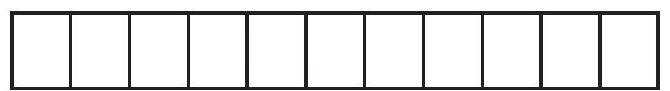
\includegraphics[max width=\textwidth, center]{2024_11_21_06df787f12c5337a1fe8g-01(1)}

PESEL ZDAJĄCEGO\\

\includegraphics[max width=\textwidth, center]{2024_11_21_06df787f12c5337a1fe8g-01}

KOD\\
ZDAJĄCEGO

\section*{ZADANIA ZAMKNIĘTE}
W zadaniach 1.-5. wybierz i zaznacz na karcie odpowiedzi jedną poprawną odpowiedź.

\section*{Zadanie 1. (0-1)}
Równanie \(\left(x^{2}+2 x-3\right)\left(x^{2}+x-m\right)=0\) ma cztery różne rozwiązania. Zatem zbiór wszystkich liczb \(m\) to:\\
A. \(\left(-\frac{1}{4},+\infty\right)\)\\
B. \(\left(-\frac{1}{4},+\infty\right) \backslash\{2,6\}\)\\
C. \(\left(-\frac{1}{4},+\infty\right) \backslash\{-2,6\}\)\\
D. \(\left(-\frac{1}{4},+\infty\right)\)

\section*{Zadanie 2. (0-1)}
Liczbę naturalną \(n\) można zapisać w postaci \(n=x^{4} y^{2}\), gdzie \(x, y\) są liczbami pierwszymi. Zatem liczba różnych dzielników naturalnych liczby \(n\) jest równa:\\
A. 15\\
B. 13\\
C. 10\\
D. 8

\section*{Zadanie 3. (0-1)}
Liczba rozwiązań równania \(\sqrt{\left(2 x^{2}+1\right)^{2}}=3\) jest równa:\\
A. 1\\
B. 2\\
C. 3\\
D. 4

\section*{Zadanie 4. (0-1)}
Reszta z dzielenia wielomianu \(W(x)\) przez dwumian \((x-1)\) jest równa 4, a reszta z dzielenia tego wielomianu przez \((x+3)\) jest równa \((-16)\). Wynika stąd, że reszta z dzielenia tego wielomianu przez \((x-1) \cdot(x+3)\) jest równa:\\
A. \(5 x+1\)\\
B. \(-5 x+1\)\\
C. \(5 x-1\)\\
D. \(-5 x-1\)

\section*{Zadanie 5. (0-1)}
Jeśli w ostrosłupie czworokątnym podstawą jest kwadrat i jedna z krawędzi bocznych o długości boku tego kwadratu jest prostopadła do płaszczyzny podstawy ostrosłupa, to cosinus kąta między ścianami bocznymi nieprostopadłymi do płaszczyzny podstawy jest równy:\\
A. \(-\frac{1}{3}\)\\
B. \(\frac{1}{3}\)\\
C. \(\frac{1}{2}\)\\
D. \(-\frac{1}{2}\)

BRUDNOPIS (nie podlega ocenie)\\

\includegraphics[max width=\textwidth, center]{2024_11_21_06df787f12c5337a1fe8g-03}

\section*{ZADANIA OTWARTE}
W zadaniach 6.-8. zakoduj wynik w kratkach zamieszczonych pod poleceniem.\\
W zadaniach 9.-18. rozwiązania należy zapisać w wyznaczonych miejscach pod treścią.

\section*{Zadanie 6. (0-2)}
Liczby rzeczywiste \(x, y\) spełniają równanie \(2 x+y-5=0\). Oblicz najmniejszą wartość wyrażenia \(W=8 x^{3}+y^{3}\). Zakoduj cyfrę dziesiątek, jedności i początkową cyfrę po przecinku rozwinięcia dziesiętnego otrzymanego wyniku.\\

\includegraphics[max width=\textwidth, center]{2024_11_21_06df787f12c5337a1fe8g-04}

\section*{Zadanie 7. (0-2)}
Dany jest trapez \(A B C D\) opisany na okręgu. Środkowa trapezu ma długość \(\frac{2}{13}\). Oblicz obwód trapezu. Zakoduj trzy początkowe cyfry po przecinku rozwinięcia dziesiętnego otrzymanego wyniku.\\

\includegraphics[max width=\textwidth, center]{2024_11_21_06df787f12c5337a1fe8g-04(1)}

\section*{Zadanie 8. (0-2)}
Dany jest okrąg o równaniu \(x^{2}+y^{2}-14 x+6 y+54=0\). Prosta \(l\) o równaniu \(y=-\frac{3}{4} x+\frac{11}{4}\) przecina ten okrąg w punktach \(A, B\). Oblicz długość cięciwy \(A B\). Zakoduj cyfrę jedności i dwie początkowe cyfry po przecinku rozwinięcia dziesiętnego otrzymanego wyniku.

\begin{center}
\begin{tabular}{|c|c|c|c|c|c|c|c|c|c|c|c|c|c|c|c|c|c|c|c|c|c|}
\hline
 &  &  &  &  &  &  &  &  &  &  &  &  &  &  &  &  &  &  &  &  &  \\
\hline
 &  &  &  &  &  &  &  &  &  &  &  &  &  &  &  &  &  &  &  &  &  \\
\hline
 &  &  &  &  &  &  &  &  &  &  &  &  &  &  &  &  &  &  &  &  &  \\
\hline
 &  &  &  &  &  &  &  &  &  &  &  &  &  &  &  &  &  &  &  &  &  \\
\hline
 &  &  &  &  &  &  &  &  &  &  &  &  &  &  &  &  &  &  &  &  &  \\
\hline
 &  &  &  &  &  &  &  &  &  &  &  &  &  &  &  &  &  &  &  &  &  \\
\hline
 &  &  &  &  &  &  &  &  &  &  &  &  &  &  &  &  &  &  &  &  &  \\
\hline
 &  &  &  &  &  &  &  &  &  &  &  &  &  &  &  &  &  &  &  &  &  \\
\hline
 &  &  &  &  &  &  &  &  &  &  &  &  &  &  &  &  &  &  &  &  &  \\
\hline
 &  &  &  &  &  &  &  &  &  &  &  &  &  &  &  &  &  &  &  &  &  \\
\hline
 &  &  &  &  &  &  &  &  &  &  &  &  &  &  &  &  &  &  &  &  &  \\
\hline
 &  &  &  &  &  &  &  &  &  &  &  &  &  &  &  &  &  &  &  &  &  \\
\hline
 &  &  &  &  &  &  &  &  &  &  &  &  &  &  &  &  &  &  &  &  &  \\
\hline
 &  &  &  &  &  &  &  &  &  &  &  &  &  &  &  &  &  &  &  &  &  \\
\hline
 &  &  &  &  &  &  &  &  &  &  &  &  &  &  &  &  &  &  &  &  &  \\
\hline
 &  &  &  &  &  &  &  &  &  &  &  &  &  &  &  &  &  &  &  &  &  \\
\hline
 &  &  &  &  &  &  &  &  &  &  &  &  &  &  &  &  &  &  &  &  &  \\
\hline
 &  &  &  &  &  &  &  &  &  &  &  &  &  &  &  &  &  &  &  &  &  \\
\hline
 &  &  &  &  &  &  &  &  &  &  &  &  &  &  &  &  &  &  &  &  &  \\
\hline
 &  &  &  &  &  &  &  &  &  &  &  &  &  &  &  &  &  &  &  &  &  \\
\hline
 &  &  &  &  &  &  &  &  &  &  &  &  &  &  &  &  &  &  &  &  &  \\
\hline
 &  &  &  &  &  &  &  &  &  &  &  &  &  &  &  &  &  &  &  &  &  \\
\hline
 &  &  &  &  &  &  &  &  &  &  &  &  &  &  &  &  &  &  &  &  &  \\
\hline
 &  &  &  &  &  &  &  &  &  &  &  &  &  &  &  &  &  &  &  &  &  \\
\hline
 &  &  &  &  &  &  &  &  &  &  &  &  &  &  &  &  &  &  &  &  &  \\
\hline
 &  &  &  &  &  &  &  &  &  &  &  &  &  &  &  &  &  &  &  &  &  \\
\hline
 &  &  &  &  &  &  &  &  &  &  &  &  &  &  &  &  &  &  &  &  &  \\
\hline
 &  &  &  &  &  &  &  &  &  &  &  &  &  &  &  &  &  &  &  &  &  \\
\hline
 &  &  &  &  &  &  &  &  &  &  &  &  &  &  &  &  &  &  &  &  &  \\
\hline
 &  &  &  &  &  &  &  &  &  &  &  &  &  &  &  &  &  &  &  &  &  \\
\hline
 &  &  &  &  &  &  &  &  &  &  &  &  &  &  &  &  &  &  &  &  &  \\
\hline
 &  &  &  &  &  &  &  &  &  &  &  &  &  &  &  &  &  &  &  &  &  \\
\hline
 &  &  &  &  &  &  &  &  &  &  &  &  &  &  &  &  &  &  &  &  &  \\
\hline
 &  &  &  &  &  &  &  &  &  &  &  &  &  &  &  &  &  &  &  &  &  \\
\hline
 &  &  &  &  &  &  &  &  &  &  &  &  &  &  &  &  &  &  &  &  &  \\
\hline
 &  &  &  &  &  &  &  &  &  &  &  &  &  &  &  &  &  &  &  &  &  \\
\hline
 &  &  &  &  &  &  &  &  &  &  &  &  &  &  &  &  &  &  &  &  &  \\
\hline
 &  &  &  &  &  &  &  &  &  &  &  &  &  &  &  &  &  &  &  &  &  \\
\hline
 &  &  &  &  &  &  &  &  &  &  &  &  &  &  &  &  &  &  &  &  &  \\
\hline
\end{tabular}
\end{center}

\section*{Zadanie 9. (0-3)}
Wykaż, że nie istnieje styczna do hiperboli o równaniu \(y=\frac{4 x}{x-3}\) prostopadła do prostej \(l\)\\
o równaniu \(2 x+4 y-1=0\).\\

\includegraphics[max width=\textwidth, center]{2024_11_21_06df787f12c5337a1fe8g-06}

Zadanie 10. (0-4)\\
Dana jest funkcja \(f\) określona wzorem \(f(x)=\frac{2 x}{x^{2}+4}\). Wyznacz zbiór wartości tej funkcji.\\

\includegraphics[max width=\textwidth, center]{2024_11_21_06df787f12c5337a1fe8g-07}

Odpowiedź:

\section*{Zadanie 11. (0-2)}
Dany jest nieskończony ciąg geometryczny \(\left(a_{n}\right)\) zbieżny o pierwszym wyrazie dodatnim. Wykaż, że suma wszystkich wyrazów tego ciągu o numerach nieparzystych jest większa lub równa od czterokrotności trzeciego wyrazu ciągu \(\left(a_{n}\right)\).\\

\includegraphics[max width=\textwidth, center]{2024_11_21_06df787f12c5337a1fe8g-08}

\section*{Zadanie 12. (0-3)}
Rozwiąż nierówność \(4 \cos ^{2} 2 x-3<0\) dla \(x \in\langle 0,2 \pi\rangle\).\\

\includegraphics[max width=\textwidth, center]{2024_11_21_06df787f12c5337a1fe8g-09}

Odpowiedź:

\section*{Zadanie 13. (0-4)}
Wyznacz liczbę dwudziestocyfrowych liczb, których suma cyfr jest równa 4.\\

\includegraphics[max width=\textwidth, center]{2024_11_21_06df787f12c5337a1fe8g-10}

Odpowiedź:

\section*{Zadanie 14. (0-4)}
Dane są punkty: \(A=(-1,-2), B=(1,4), C=(-2,-10), D=(2,2)\). Wykaż, że odcinki \(A B\) i \(C D\) są równoległe. Wyznacz środek jednokładności \(S\) i dodatnią skalę \(k\) tak, aby obrazem odcinka \(A B\) w tej jednokładności był odcinek \(C D\).

\begin{center}
\begin{tabular}{|c|c|c|c|c|c|c|c|c|c|c|c|c|c|c|c|c|c|c|c|c|c|}
\hline
 &  &  &  &  &  &  &  &  &  &  &  &  &  &  &  &  &  &  &  &  &  \\
\hline
 &  &  &  &  &  &  &  &  &  &  &  &  &  &  &  &  &  &  &  &  &  \\
\hline
 &  &  &  &  &  &  &  &  &  &  &  &  &  &  &  &  &  &  &  &  &  \\
\hline
 &  &  &  &  &  &  &  &  &  &  &  &  &  &  &  &  &  &  &  &  &  \\
\hline
 &  &  &  &  &  &  &  &  &  &  &  &  &  &  &  &  &  &  &  &  &  \\
\hline
 &  &  &  &  &  &  &  &  &  &  &  &  &  &  &  &  &  &  &  &  &  \\
\hline
 &  &  &  &  &  &  &  &  &  &  &  &  &  &  &  &  &  &  &  &  &  \\
\hline
 &  &  &  &  &  &  &  &  &  &  &  &  &  &  &  &  &  &  &  &  &  \\
\hline
 &  &  &  &  &  &  &  &  &  &  &  &  &  &  &  &  &  &  &  &  &  \\
\hline
 &  &  &  &  &  &  &  &  &  &  &  &  &  &  &  &  &  &  &  &  &  \\
\hline
 &  &  &  &  &  &  &  &  &  &  &  &  &  &  &  &  &  &  &  &  &  \\
\hline
 &  &  &  &  &  &  &  &  &  &  &  &  &  &  &  &  &  &  &  &  &  \\
\hline
 &  &  &  &  &  &  &  &  &  &  &  &  &  &  &  &  &  &  &  &  &  \\
\hline
 &  &  &  &  &  &  &  &  &  &  &  &  &  &  &  &  &  &  &  &  &  \\
\hline
 &  &  &  &  &  &  &  &  &  &  &  &  &  &  &  &  &  &  &  &  &  \\
\hline
 &  &  &  &  &  &  &  &  &  &  &  &  &  &  &  &  &  &  &  &  &  \\
\hline
 &  &  &  &  &  &  &  &  &  &  &  &  &  &  &  &  &  &  &  &  &  \\
\hline
 &  &  &  &  &  &  &  &  &  &  &  &  &  &  &  &  &  &  &  &  &  \\
\hline
 &  &  &  &  &  &  &  &  &  &  &  &  &  &  &  &  &  &  &  &  &  \\
\hline
 &  &  &  &  &  &  &  &  &  &  &  &  &  &  &  &  &  &  &  &  &  \\
\hline
 &  &  &  &  &  &  &  &  &  &  &  &  &  &  &  &  &  &  &  &  &  \\
\hline
 &  &  &  &  &  &  &  &  &  &  &  &  &  &  &  &  &  &  &  &  &  \\
\hline
 &  &  &  &  &  &  &  &  &  &  &  &  &  &  &  &  &  &  &  &  &  \\
\hline
 &  &  &  &  &  &  &  &  &  &  &  &  &  &  &  &  &  &  &  &  &  \\
\hline
 &  &  &  &  &  &  &  &  &  &  &  &  &  &  &  &  &  &  &  &  &  \\
\hline
 &  &  &  &  &  &  &  &  &  &  &  &  &  &  &  &  &  &  &  &  &  \\
\hline
 &  &  &  &  &  &  &  &  &  &  &  &  &  &  &  &  &  &  &  &  &  \\
\hline
 &  &  &  &  &  &  &  &  &  &  &  &  &  &  &  &  &  &  &  &  &  \\
\hline
 &  &  &  &  &  &  &  &  &  &  &  &  &  &  &  &  &  &  &  &  &  \\
\hline
 &  &  &  &  &  &  &  &  &  &  &  &  &  &  &  &  &  &  &  &  &  \\
\hline
 &  &  &  &  &  &  &  &  &  &  &  &  &  &  &  &  &  &  &  &  &  \\
\hline
 &  &  &  &  &  &  &  &  &  &  &  &  &  &  &  &  &  &  &  &  &  \\
\hline
 &  &  &  &  &  &  &  &  &  &  &  &  &  &  &  &  &  &  &  &  &  \\
\hline
 &  &  &  &  &  &  &  &  &  &  &  &  &  &  &  &  &  &  &  &  &  \\
\hline
 &  &  &  &  &  &  &  &  &  &  &  &  &  &  &  &  &  &  &  &  &  \\
\hline
 &  &  &  &  &  &  &  &  &  &  &  &  &  &  &  &  &  &  &  &  &  \\
\hline
 &  &  &  &  &  &  &  &  &  &  &  &  &  &  &  &  &  &  &  &  &  \\
\hline
 &  &  &  &  &  &  &  &  &  &  &  &  &  &  &  &  &  &  &  &  &  \\
\hline
 &  &  &  &  &  &  &  &  &  &  &  &  &  &  &  &  &  &  &  &  &  \\
\hline
\end{tabular}
\end{center}

Odpowiedź:

\section*{Zadanie 15. (0-4)}
Dany jest ostrosłup prawidłowy trójkątny, w którym długość krawędzi podstawy jest równa \(a\), a krawędź boczna jest nachylona do płaszczyzny podstawy pod kątem \(\alpha\). Ostrosłup ten przecięto płaszczyzną, która przechodzi przez krawędź podstawy i jest nachylona do płaszczyzny podstawy ostrosłupa pod kątem \(\frac{\alpha}{2}\). Oblicz pole otrzymanego przekroju.\\

\includegraphics[max width=\textwidth, center]{2024_11_21_06df787f12c5337a1fe8g-12}

Odpowiedź:

\section*{Zadanie 16. (0-4)}
W urnie I jest 7 czarnych kul, a w urnie II są 3 czarne kule. Do tych urn wkładamy losowo w sumie 3 kule białe. Następnie losujemy urnę i z urny jedną kulę. Oblicz, ile należy wrzucić białych kul do urny I, aby prawdopodobieństwo wylosowania białej kuli z losowo wybranej urny było równe \(\frac{17}{72}\).\\

\includegraphics[max width=\textwidth, center]{2024_11_21_06df787f12c5337a1fe8g-13}

Odpowiedź:

\section*{Zadanie 17. (0-4)}
Dane jest równanie \(x^{2}+(2 m+1) x-3 m^{2}-\frac{1}{2} m+\frac{1}{4}=0\). Wyznacz zbiór wszystkich wartości parametru wartości parametru \(m\), dla których to równanie ma dokładnie dwa różne rozwiązania mniejsze od 4.\\

\includegraphics[max width=\textwidth, center]{2024_11_21_06df787f12c5337a1fe8g-14}

Zadanie 18. (0-7)\\
W okrąg o promieniu \(R\) wpisano prostokąt \(A B C D\). Wyznacz możliwie największe pole tego prostokąta.

\begin{center}
\begin{tabular}{|c|c|c|c|c|c|c|c|c|c|c|c|c|c|c|c|c|c|c|c|c|c|}
\hline
 &  & - &  &  &  &  &  &  &  &  &  &  &  &  &  &  &  &  &  &  &  \\
\hline
 &  &  &  &  &  &  &  &  &  &  &  &  &  &  &  &  &  &  &  &  &  \\
\hline
 &  &  &  &  &  &  &  &  &  &  &  &  &  &  &  &  &  &  &  &  &  \\
\hline
 &  &  &  &  &  &  &  &  &  &  &  &  &  &  &  &  &  &  &  &  &  \\
\hline
 &  &  &  &  &  &  &  &  &  &  &  &  &  &  &  &  &  &  &  &  &  \\
\hline
 &  &  &  &  &  &  &  &  &  &  &  &  &  &  &  &  &  &  &  &  &  \\
\hline
 &  &  &  &  &  &  &  &  &  &  &  &  &  &  &  &  &  &  &  &  &  \\
\hline
 &  &  &  &  &  &  &  &  &  &  &  &  &  &  &  &  &  &  &  &  &  \\
\hline
 &  &  &  &  &  &  &  &  &  &  &  &  &  &  &  &  &  &  &  &  &  \\
\hline
 &  &  &  &  &  &  &  &  &  &  &  &  &  &  &  &  &  &  &  &  &  \\
\hline
 &  &  &  &  &  &  &  &  &  &  &  &  &  &  &  &  &  &  &  &  &  \\
\hline
 &  &  &  &  &  &  &  &  &  &  &  &  &  &  &  &  &  &  &  &  &  \\
\hline
 &  &  &  &  &  &  &  &  &  &  &  &  &  &  &  &  &  &  &  &  &  \\
\hline
 &  &  &  &  &  &  &  &  &  &  &  &  &  &  &  &  &  &  &  &  &  \\
\hline
 &  &  &  &  &  &  &  &  &  &  &  &  &  &  &  &  &  &  &  &  &  \\
\hline
 &  &  &  &  &  &  &  &  &  &  &  &  &  &  &  &  &  &  &  &  &  \\
\hline
 &  &  &  &  &  &  &  &  &  &  &  &  &  &  &  &  &  &  &  &  &  \\
\hline
 &  &  &  &  &  &  &  &  &  &  &  &  &  &  &  &  &  &  &  &  &  \\
\hline
 &  &  &  &  &  &  &  &  &  &  &  &  &  &  &  &  &  &  &  &  &  \\
\hline
 &  &  &  &  &  &  &  &  &  &  &  &  &  &  &  &  &  &  &  &  &  \\
\hline
 &  &  &  &  &  &  &  &  &  &  &  &  &  &  &  &  &  &  &  &  &  \\
\hline
 &  &  &  &  &  &  &  &  &  &  &  &  &  &  &  &  &  &  &  &  &  \\
\hline
 &  &  &  &  &  &  &  &  &  &  &  &  &  &  &  &  &  &  &  &  &  \\
\hline
 &  &  &  &  &  &  &  &  &  &  &  &  &  &  &  &  &  &  &  &  &  \\
\hline
 &  &  &  &  &  &  &  &  &  &  &  &  &  &  &  &  &  &  &  &  &  \\
\hline
 &  &  &  &  &  &  &  &  &  &  &  &  &  &  &  &  &  &  &  &  &  \\
\hline
 &  &  &  &  &  &  &  &  &  &  &  &  &  &  &  &  &  &  &  &  &  \\
\hline
 &  &  &  &  &  &  &  &  &  &  &  &  &  &  &  &  &  &  &  &  &  \\
\hline
 &  &  &  &  &  &  &  &  &  &  &  &  &  &  &  &  &  &  &  &  &  \\
\hline
 &  &  &  &  &  &  &  &  &  &  &  &  &  &  &  &  &  &  &  &  &  \\
\hline
 &  &  &  &  &  &  &  &  &  &  &  &  &  &  &  &  &  &  &  &  &  \\
\hline
 &  &  &  &  &  &  &  &  &  &  &  &  &  &  &  &  &  &  &  &  &  \\
\hline
 &  &  &  &  &  &  &  &  &  &  &  &  &  &  &  &  &  &  &  &  &  \\
\hline
 &  &  &  &  &  &  &  &  &  &  &  &  &  &  &  &  &  &  &  &  &  \\
\hline
 &  &  &  &  &  &  &  &  &  &  &  &  &  &  &  &  &  &  &  &  &  \\
\hline
 &  &  &  &  &  &  &  &  &  &  &  &  &  &  &  &  &  &  &  &  &  \\
\hline
 &  &  &  &  &  &  &  &  &  &  &  &  &  &  &  &  &  &  &  &  &  \\
\hline
 &  &  &  &  &  &  &  &  &  &  &  &  &  &  &  &  &  &  &  &  &  \\
\hline
 &  &  &  &  &  &  &  &  &  &  &  &  &  &  &  &  &  &  &  &  &  \\
\hline
 &  &  &  &  &  &  &  &  &  &  &  &  &  &  &  &  &  &  &  &  &  \\
\hline
 &  &  &  &  &  &  &  &  &  &  &  &  &  &  &  &  &  &  &  &  &  \\
\hline
\end{tabular}
\end{center}

Odpowiedź:

\section*{BRUDNOPIS (nie podlega ocenie)}
\begin{center}

\includegraphics[max width=\textwidth]{2024_11_21_06df787f12c5337a1fe8g-16}
\end{center}


\end{document}